%!TEX root = ../main.tex

\section{$B^- \rightarrow D^0$ control decay}
\label{sec:chargedCorrBtoD0}

To monitor the analysis steps, which are applied to both measured and simulated data, a control decay of the form \\
%\vspace{0.1 cm}\\
\begin{center}
 $B^+ \rightarrow D^0 X$, $D^0 \rightarrow K^+ \pi^-$ 
\end{center}
%\vspace{0.1 cm}
is used. The statistics is much more abundant for this channel.

\subsection{Dataset used}

For this analysis the amount of data and Monte Carlo simulated data used was restricted to the SVD2 period: experiments ranging from 31 to 65. This choice was made to save processing time, anyway most of the $B\bar{B}$ meson pairs were produced in this range of experiments (620 $\times 10^6$ out of almost 800 $\times 10^6$ ).

\subsection{Event selection and reconstruction}

The approach used for the inclusive decays reconstruction is the same as for the $B \rightarrow \Lambda_c$ analysis. The same FEI training was used, though excluding the signal decay $D^0 \rightarrow K^+ \pi^-$ from the decay chains used by the FEI to reconstruct the $B_{tag}$.
Same preliminary selection criteria were applied to the tag-side $B$ meson candidates as well. \\
\noindent In the \textit{rest of event} (ROE) of the reconstructed $B_{tag}$ meson, to select $D^0 \rightarrow K^+ \pi^-$ signal candidates, the following event selection criteria are applied:
\begin{itemize}
\item $dr <$ 2 cm and $|dz| <$ 4 cm
\item $\frac{\mathcal{L}_{K}}{\mathcal{L_{K}}+\mathcal{L_{\pi}}} > 0.6$
\end{itemize}
For the $D^0 $ candidates a vertex fit is performed with \texttt{TreeFitter}, requiring it to converge.  If there are more than one $D^0$ combination, then the best candidate based on the $\chi^2$ probability is chosen. The $D^0$ signal region is defined to be $|M_{D^0}  - m_{D^0}| < $   30  MeV/$c^2$ 
\newline \noindent ($\sim$ 3$\sigma$), where $m_{D^0 }$ is the nominal mass of $D^0$.\\
\subsection{Signal selection optimization}\label{Sec:SigSelectionOpt}

Following the same procedure as for the $B \rightarrow \Lambda_c$ analysis, the optimized selection cuts obtained for the event based ratio
of the 2-nd to the 0-th order Fox-Wolfram moments, the $B_{tag}$ signal probability and the momentum of the $D^0$ candidates in the center of mass system are\footnote{illustrative plots can be found in Appendix \ref{chargedBtoD0App}}:
\begin{itemize}
\item $foxWolframR2 <$ 0.3
\item SignalProbability $>$ 0.004
\item $p^{D^0 }_{CMS} > 1$ GeV/c$^2$
\end{itemize}

 \noindent Figure \ref{fig:chargedControlD0_Mbc_InvM_opt_SignalRegion} shows the distributions of $M_{bc}$ and invariant mass in the signal region\footnote{signal region: $M_{bc}  > $ 5.27 GeV/c$^2$ and $|M_{D^0}  - m_{D^0}| < $   30  MeV/$c^2$}  for the $B^- \rightarrow D^0 X$ reconstructed events after the selection cuts were applied.

\begin{figure}[h!]
\centering
{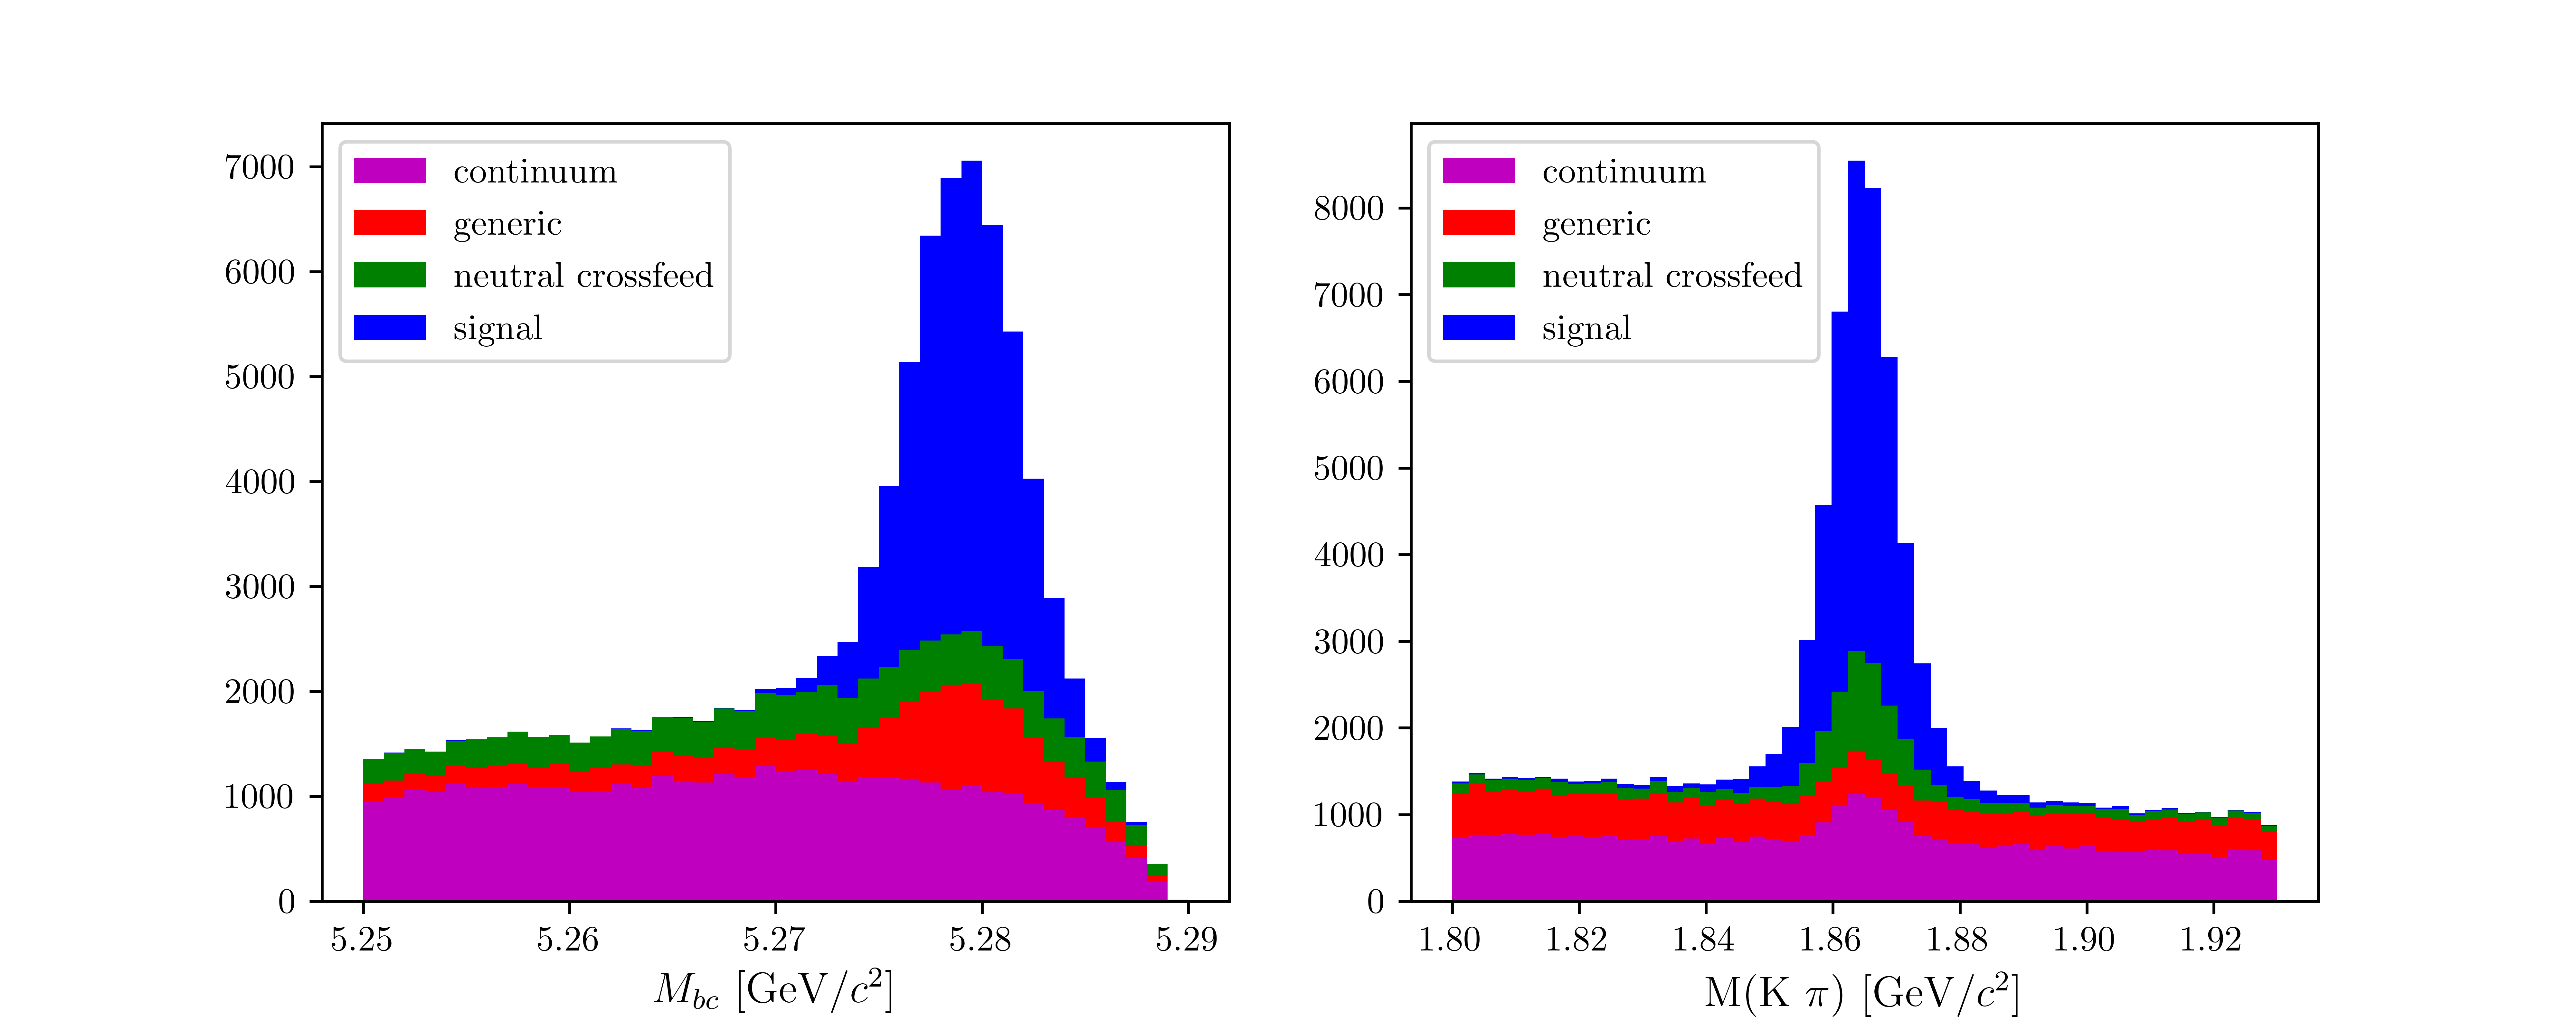
\includegraphics[width=1.2\textwidth]{05-chargedControlSample/figs/rel5_chargedBtoD0bar_Mbc_InvM_opt_SigRegion.png}}
\caption{Distribution of $M_{bc}$ (left) and invariant mass of charged correlated  $D^0 $ candidates (right), in the signal region after the above mentioned selection cuts.}
\label{fig:chargedControlD0_Mbc_InvM_opt_SignalRegion}
\end{figure}

\vspace{1 cm}

\subsection{Probability Density Functions (PDFs) for two dimensional fit}

As already said the main goal of the control sample analysis is to ensure that the method used to extract the signal yields discriminating the correctly reconstructed from the misreconstructed signal events by fitting is valid.
The reconstructed events in $M_{bc}$ are fitted with a Crystal Ball, the misreconstructed signal with a Novosibirsk function. As in the $B \rightarrow \Lambda_c$ analysis both components have a correspondent peak in the $D^0$ mass which 
is fitted with a sum of three gaussians with a common mean.
The fitted distribution of $M_{bc}$ and $M(\pi K)$ are shown in Fig. \ref{fig:chargedTotalSignal2Dfit} with signal MC sample. 

\begin{figure}[H]
%\centering
{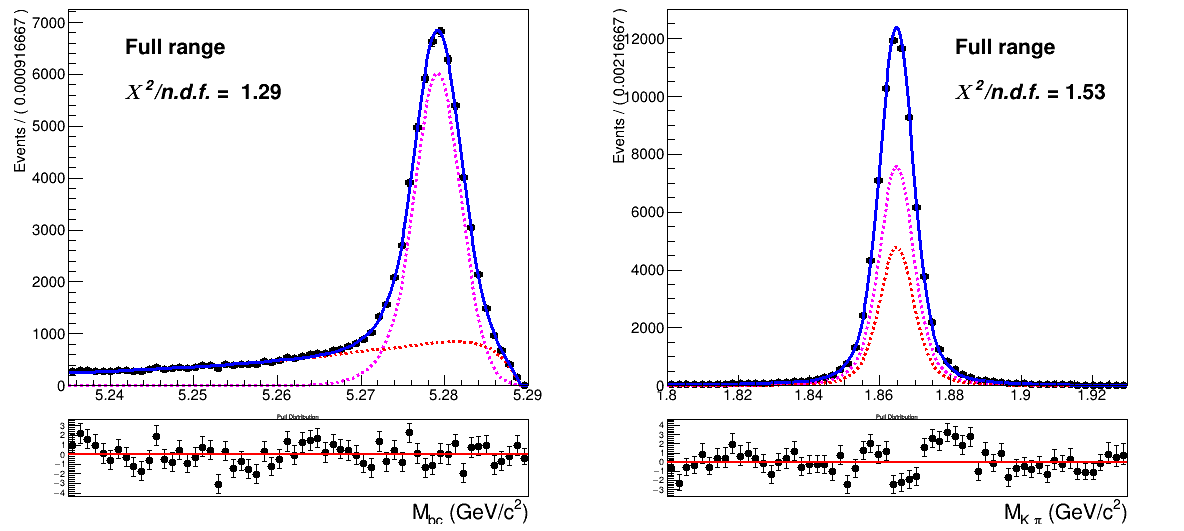
\includegraphics[width=0.90\textwidth]{05-chargedControlSample/figs/TotalSignal2Dfit_Mbc_free_Novosibirsk_and_CB_w_sig_frac.png}}
\caption{Two dimensional fit of total signal events in $M_{bc}$  and $M(p K \pi)$ (in magenta reconstructed signal PDF, misreconstructed signal PDF in red)}
\label{fig:chargedTotalSignal2Dfit}
\end{figure}

As already seen in the $B \rightarrow \Lambda_c$ analysis  besides the misreconstructed signal the other background components are:

\begin{itemize}
    \item \textbf{generic} (charged $B$) background
    \item \textbf{crossfeed} (neutral $B$) background 
    \item \textbf{continuum} background 
\end{itemize}
\vspace{0.2 cm}
\noindent \textbf{Generic background}

\noindent The generic background deriving from other $B^+B^-$ events presents a similar shape in $M_{bc}$: it is fitted again with a sum of Crystal Ball and Novosibirsk function. Instead the distribution in  the $D^0$ mass  is fitted with a sum of first order Polynomial function and a small gaussian peak, which is due to the small 
amount of flavor anti-correlated $B^+ \rightarrow D^0$ reconstructed events (see Fig. \ref{fig:chargedControlD0_Generic_2DFit}). The total two-dimensional PDF is a product of the one-dimensional PDFs in $M_{bc}$ and $D^0$ mass:

\begin{equation}
P^{GenBkg}_{B,D^0}(M_{bc}, M(K \pi)) = [\Gamma_{CB}(M_{bc}) + \Gamma_{Nov}(M_{bc})] \times [\rho_{pol1}(M(K \pi)+ \rho_{G}(M(K \pi))
 \end{equation}



\begin{figure}[H]
%\centering
{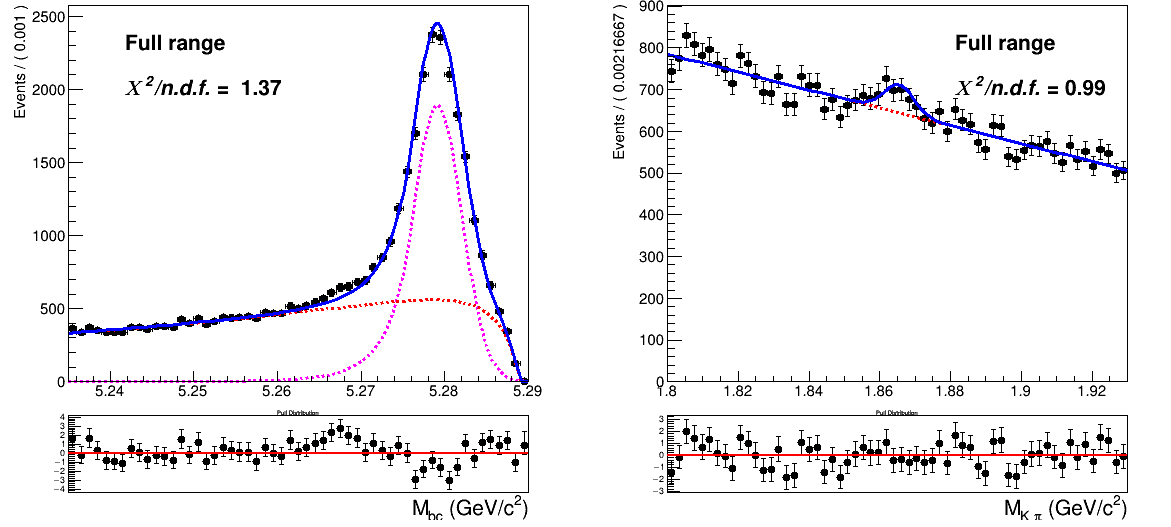
\includegraphics[width=0.90\textwidth]{05-chargedControlSample/figs/chargedControlD0_Generic_2DFit.png}}
\caption{Two dimensional fit of generic ($B^+B^-$) background events in $M_{bc}$  and $M(K \pi)$.}
\label{fig:chargedControlD0_Generic_2DFit}
\end{figure}

\noindent \textbf{Crossfeed background}
\noindent The crossfeed background deriving from $B^0\bar{B^0}$ events is shown in Fig. \ref{fig:chargedControlD0_NeutralCrossfeed_2DFit} 
The $M_{bc}$  distribution is fitted with a sum of Novosibirsk and Argus functions.
The distribution in the $D^0$ mass is fitted with a first order Chebyshev polynomial and the $D^0$ mass peak is fitted with the same sum of three gaussians used to describe the signal peak (same parametrization used already in $\BtoLambda$ analysis).

\begin{figure}[h!]
{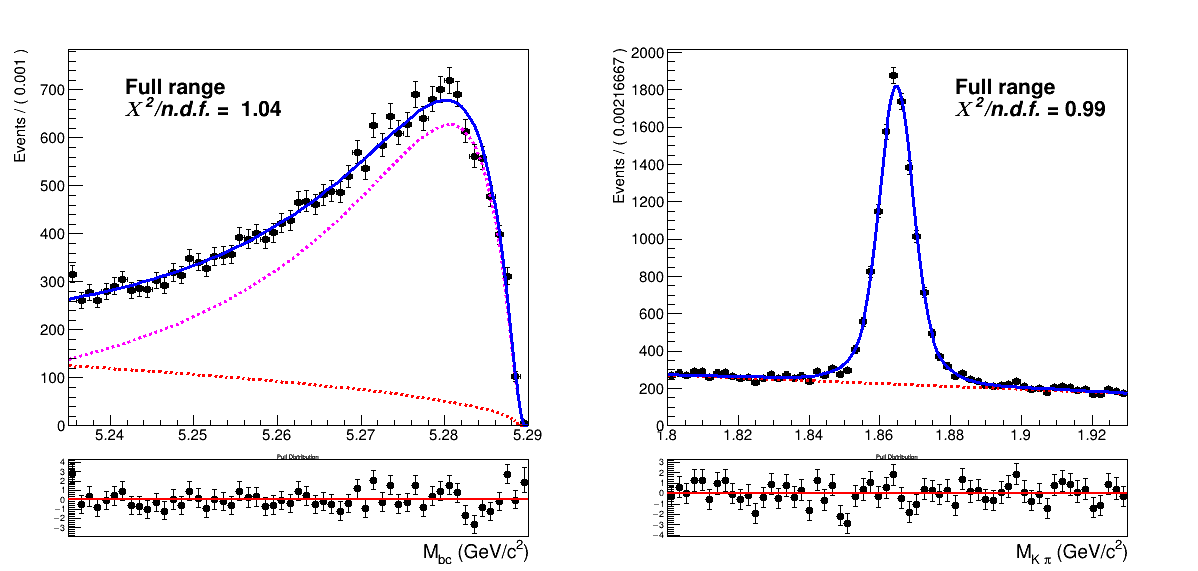
\includegraphics[width=0.90\textwidth]{05-chargedControlSample/figs/NEW_chargedControlD0_NeutralCrossfeed_2DFit_.png}}
\caption{Two dimensional fit of crossfeed ($B^0\bar{B^0}$) events in $M_{bc}$  and $M(K \pi)$.}
\label{fig:chargedControlD0_NeutralCrossfeed_2DFit}
\end{figure}

\noindent \textbf{Continuum background}
\newline
\noindent The procedure adopted to model the continuum background is the same used for the $B \rightarrow \Lambda_c$ decays, but in this case
the available statistics is enough to perform the scaling with all the selection cuts also in the case of the two-dimensional fit (not removing the continuum suppression).

  
 \begin{figure}[H]
 \centering
\subcaptionbox{\label{fig:chargedControlD0_2Dcontinuum_on-offMbc}}
{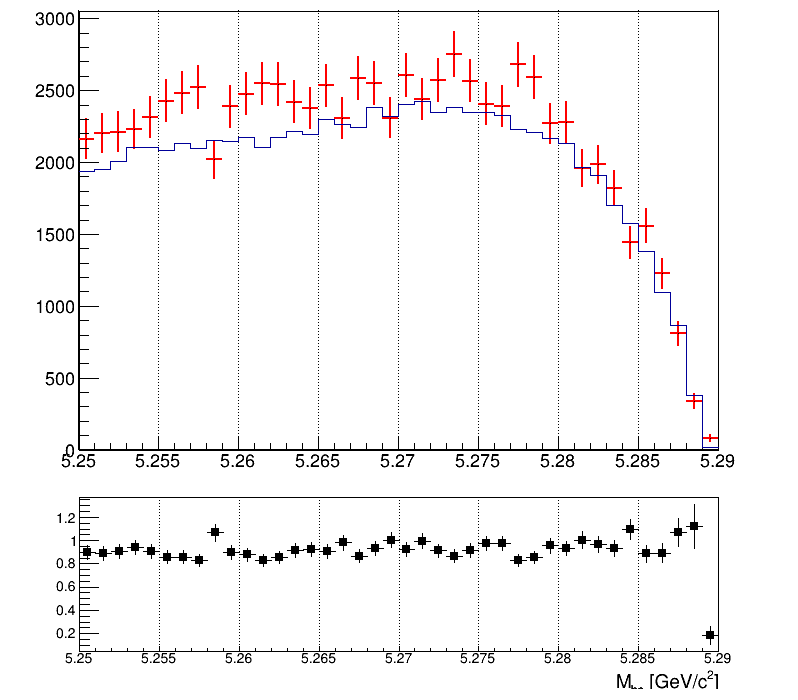
\includegraphics[width=.45\textwidth]{05-chargedControlSample/figs/on_off_res_chargedControlD0_Mbc.png}}
\subcaptionbox{\label{fig:chargedControlD0_corrected_2DcontinuumMbc}}
{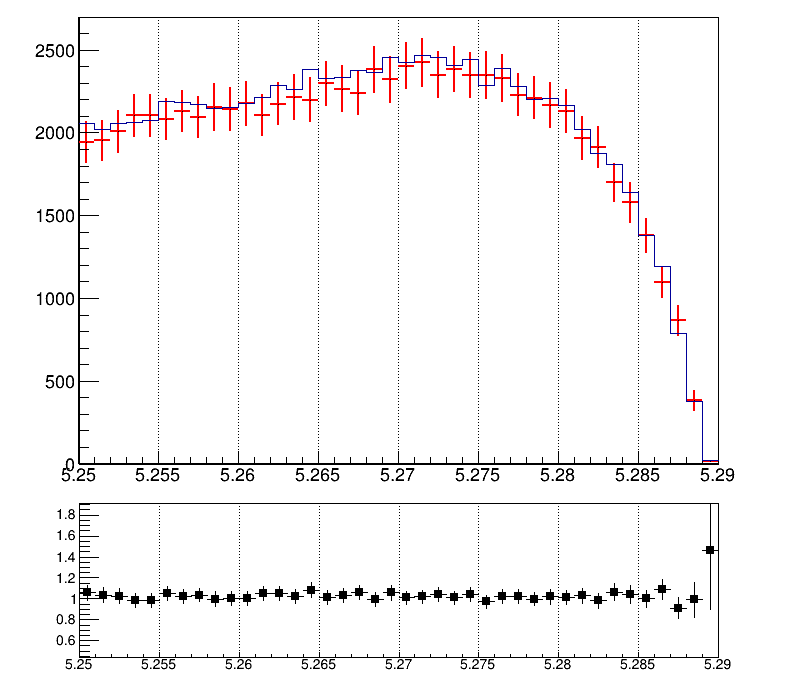
\includegraphics[width=.45\textwidth]{05-chargedControlSample/figs/chargedControlD0_corrected_2DcontinuumMbc.png}}
\caption{In \cref{fig:chargedControlD0_2Dcontinuum_on-offMbc} $M_{bc}$ distributions of the MC (scaled) off-resonance sample (in red) and on-resonance (in blue).  In \cref{fig:chargedControlD0_corrected_2DcontinuumMbc} $M_{bc}$ distributions of the corrected scaled off-resonance and on-resonance MC continuum.}
\end{figure}

\noindent For each bin a correction factor is calculated, in order to have a reasonable match with the expected continuum background. Fig. \ref{fig:chargedControlD0_corrected_2DcontinuumMbc} shows the applied correction on an independent MC sample.
As in the case of $B \rightarrow \Lambda_c$ analysis, then the resulting $M_{bc}$ distribution is fitted with a Novosibirsk function , whereas the $D^0$ mass distribution is fitted with a sum of first order Chebyshev polynomial and the sum of three gaussians used to describe the signal peak (as shown in \cref{fig:InvMchargedControlD0_off-resonanceMC_rescaled_2Dfit_w_peak_frac}). The fraction of events in the peak is the same in on- and off-resonance MC. This method is applied also to scale the off-resonance data.

\begin{figure}[H]
\centering
{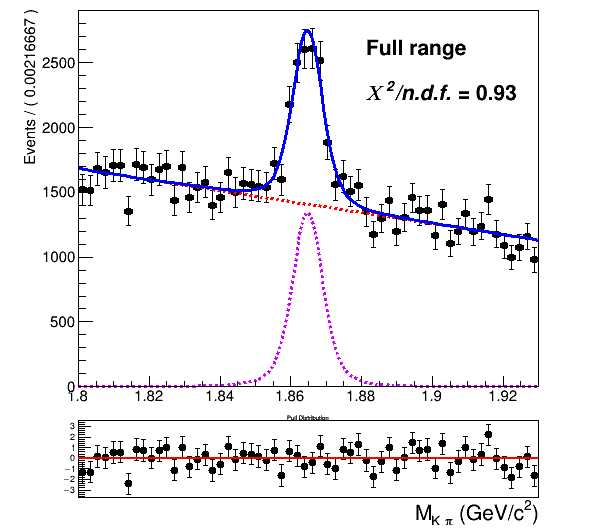
\includegraphics[width=0.40\textwidth]{05-chargedControlSample/figs/InvMchargedControlD0_off-resonanceMC_rescaled_2Dfit_w_peak_frac.png}}
\caption{$D^0$ mass fit of scaled off-resonance  Monte Carlo}
\label{fig:InvMchargedControlD0_off-resonanceMC_rescaled_2Dfit_w_peak_frac}
\end{figure}

\subsection{2D Fit on Monte Carlo simulated data}\label{2Dfit_chargedControlD0_onMC}

As in the $\BtoLambda$ study, five streams of Monte Carlo simulated data have been used to get values for the shaping parameters for the individidual components described in the previous section and the fit model is tested on 
an independent stream.
%In all six fits all the shaping parameters are kept fixed, except:
%\begin{itemize}
%    \item $\sigma_{G1}$: the width of the wider of the three Gaussian functions in $\rho_G(M(p K \pi))$
%    \item $\sigma_{CB}$ parameter for the Crystal Ball describing the signal
%\end{itemize}
 
For the six fits, the same conditions were applied to the widths:
\begin{itemize}
      \item $\sigma_{G1}$: the width of the wider of the three Gaussian functions in $\rho_G(M(K \pi))$
      \item $\sigma_{CB}$ parameter for the Crystal Ball describing the signal
      \item the $\sigma_{CB}$ parameter for the Crystal Ball describing the generic background is expressed as function of the signal $\sigma_{CB}$  with a ratio fixed from the MC. 
\end{itemize}

For the fits on Monte Carlo simulated data the crossfeed normalization is expressed as ratio of its contribution  and the misreconstructed signal as found in MC and kept fixed (to see how the parametrized form impacts a fit on data is then performed).
Exemplary, the distributions of stream 0 overlaid by the fitted PDF are depicted in \cref{fig:stream0_chargedControlD0_Total_2DFit} (see Appendix \ref{chargedBtoD0App} for the projections of signal regions and sidebands). 
%(floated parameters and fixed width ratios) were applied as to the two dimensional fit in the case of the \BtoLambda study.
%Those conditions are the same used ofr the  
 %Figures \ref{fig:stream0_chargedControlD0_Total_2DFit} - \ref{fig:stream4_chargedControlD0_Total_2DFit} show the fits of the 5 streams used to obtain the shaping parameters of the PDFs.

%\newpage 
In Table \ref{tab:5streams_chargedSignalYields} the yields for reconstructed and misreconstructed signal are listed for each stream.\\
%\vspace{0.1 cm}
\begin{table}[H]
\centering
%\resizebox{0.8\textwidth}{!}{%
\begin{tabular}{ |p{1.5cm}||p{2.2cm}| p{2.2cm}| p{2.2cm}| p{2.2cm}| p{2.2cm}| p{2.2cm}|  }
 \hline
  stream   &  0  & 1 & 2 & 3 & 4 & 5 \\
 \hline
 NrecSig  &  56986 $\pm$ 400  & 57766 $\pm$ 437  & 55607 $\pm$ 426 & 57068 $\pm$ 372 & 58385 $\pm$ 369 & 57501 $\pm$ 437 \\
 NmisSig &  31453 $\pm$ 321 & 30513 $\pm$ 350 & 32580  $\pm$ 350 & 33340 $\pm$  399 & 29966  $\pm$ 390 & 32012 $\pm$ 355\\
 %Generic & 36191 $\pm$ 436 &  33432 $\pm$ 439 & 37223 $\pm$ 446 &  37015  $\pm$ 388 & 34079  $\pm$ 382\\
 \hline
 \end{tabular}%
%}%
 \caption{reconstructed and misreconstructed signal yields obtained fitting 6 independent streams}\label{tab:5streams_chargedSignalYields}
\end{table}
%\vspace{0.5 cm}

To be sure that the PDFs enables us to extract the signal yield in an unbiased way, the sum of reconstructed and misreconstructed signal yields, i.e. total signal, from the fits are compared to the true values of each stream (\cref{tab:5streams_chargedTotalSignalYields}).
There are quite some differences between the fitted signal yield and the true values in individual streams. However,  all these deviations are within statistical expectations. \\

\vspace{0.5 cm}
%Total Signal:
\begin{table}[H]
\centering
\begin{tabular}{c c c c c}% |p{2cm}||p{2.5cm}| p{2.5cm}| p{2.5cm}| p{2.5cm}|   p{4cm}| }
 \hline
  streams   &  fit  & MC truth  &\multicolumn{2}{c}{fit - MC truth}  \\
 \hline
 stream 0 &  88439  $\pm$ 340  & 88144  & + 295 & (+0.33$\%$)  \\
 stream 1 &  88279 $\pm$ 361 & 88551 & $ - 272$ & (- 0.31$\%$)\\
 stream 2  & 88187 $\pm$ 360 &  88487 & -300 & (- 0.34$\%$)  \\
  stream 3  & 90408 $\pm$ 372 &  90149  &   + 259 & (+ 0.29$\%$) \\
   stream 4  & 88351 $\pm$ 383 &  87981  &  + 370 & (+ 0.42$\%$) \\
stream 5  & 89513 $\pm$ 366 &  89710  &  -197 & (- 0.22$\%$) \\
    \hline
     sum  & 533177  &  533022  & +155 & (+0.03$\%$)  \\  
 \hline 
\end{tabular}
\caption{Comparison of fitted and truth-matched total signal events in each stream.}\label{tab:5streams_chargedTotalSignalYields}
\end{table}


\begin{figure}[H]
\centering
{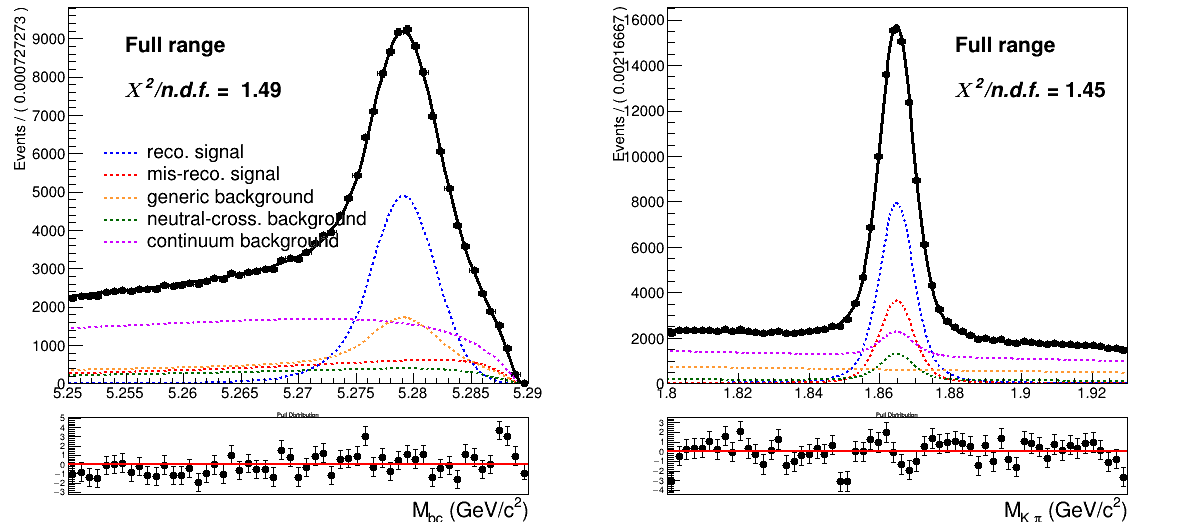
\includegraphics[width=0.85\textwidth]{05-chargedControlSample/figs/stream0_chargedControlD0_Total_2DFit.png}}
\caption{Two dimensional fit on stream 0 Monte Carlo simulated data.}
\label{fig:stream0_chargedControlD0_Total_2DFit}
\end{figure}

\subsection{2D Fit on data}\label{chargedBtoD0_2Dfit_onData}
 After obtaining the model for the continuum background scaling and correcting the $M_{bc}$ distribution of the off-resonance data, the model tested on Monte Carlo simulated data is applied on data with same free parameters and yields. \cref{fig:chargedControlD0_Total_2DFit_onData_free_sigmaCB1_InvMsigma} shows the projections of the two dimensional fit (see Appendix \ref{chargedBtoD0App} for the projections of signal regions and sidebands).
\begin{figure}[h!]
%\centering
{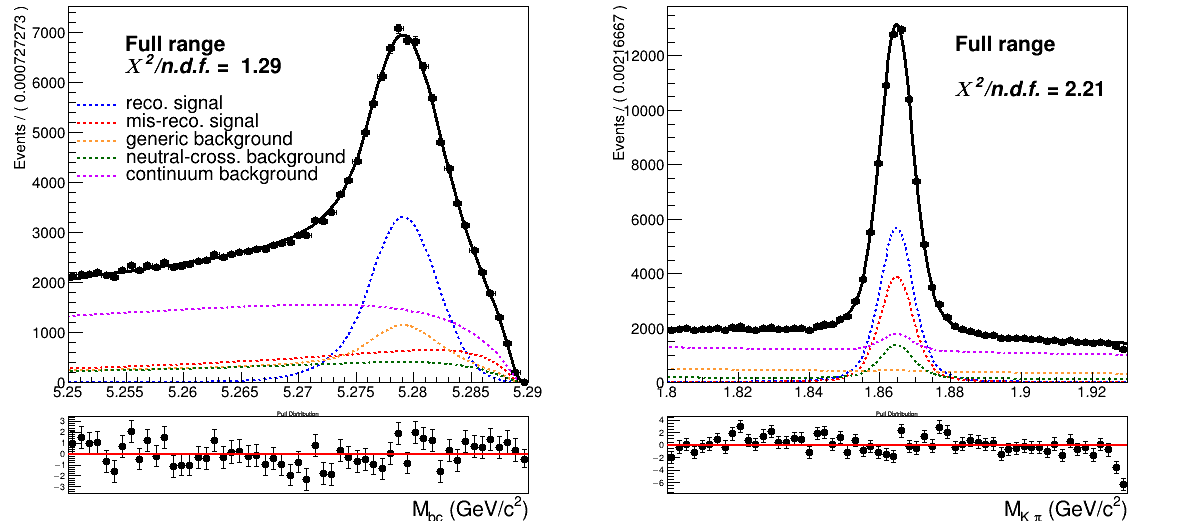
\includegraphics[width=0.80\textwidth]{05-chargedControlSample/figs/chargedControlD0_Total_2DFit_onData_free_sigmaCB1_InvMsigma.png}}
\caption{Two dimensional fit on Data (same conditions applied as in \cref{fig:stream0_chargedControlD0_Total_2DFit})}
\label{fig:chargedControlD0_Total_2DFit_onData_free_sigmaCB1_InvMsigma}
\end{figure}

\noindent Yields for the reconstructed and misreconstructed signal and for generic background are obtained from the fit: \\
 .
 \newline  \hspace{3.5 cm}
\begin{tabular}{ |p{3cm}||p{3cm}|  }

 \hline
 NrecSig  &  35629 $\pm$ 368\\
 NmisSig &  24425 $\pm$ 311 \\
 Generic & 24596 $\pm$ 407\\
 \hline
\end{tabular}
\newline
\vspace{1.5 cm}

\noindent  The total normalization from the fit is 174230 $\pm$  407 (to be compared with the total data events: 173964).\\
\vspace{0.5 cm}
 \begin{table}
\begin{tabular}{ |p{3cm}||p{3cm}| p{3cm}|  }

 \hline
 ratio        &          MC      &    DATA   \\
 \hline
 \hline
NmisSig/NrecSig  &  0.56 $\pm$ 0.01  & 0.68 $\pm$ 0.01\\
NmisSig/Generic  &  0.90 $\pm$ 0.02 &  0.99 $\pm$ 0.02  \\
Generic/NrecSig & 0.62 $\pm$ 0.01 & 0.69 $\pm$ 0.02\\
 \hline

\end{tabular}
 \caption{Comparison of ratios of yields from the two dimensional fits on Monte Carlo simulated data and on Data.} 
 \end{table}

 \noindent Since in the case of the two dimensional fit for the measurement of $B^- \rightarrow \Lambda_c^+ X$ decays the crossfeed normalization was parametrized in the form described 
 by \cref{eq:paramCrossfeedNorm}, the 2D fit shown above is repeated with the parametrized normalization for the crossfeed background. The signal reconstruction efficiency  that enters the formula to estimate the true number of 
 signal events ( $ N_{sig}  =  N_{recSig} / \epsilon$ ) is now the signal reconstruction efficiency on data: $\epsilon_{data}$. It can be estimated scaling the one found on Monte Carlo by a correction factor that takes into account the different 
 FEI efficiency on data and the signal-side reconstruction corrected for the different PID efficiency (see \cref{sec:ControlPIDeff}-\cref{sec:ControlRecoEff}), $\epsilon_{data} = \epsilon_{MC} \cdot c_{FEI} \cdot c_{D^0} = (0.216 \pm 0.016)\% $. \\

 where $c_{FEI} = 0.810_{-0.012}^{+0.013} \pm 0.054$ is the correction factor for the FEI efficiency determined in \cite{schwab_judith_2017_21422} \\
 whereas the factor $c_{D^0}$ is the PID correction reported in \cref{sec:ControlPIDeff}.\\
 \noindent \cref{fig:chargedControlD0_Total_2DFit_onData_paramCrossfeedRatio} shows this second fit.
 
 \newpage
 \noindent In the following table yields for the reconstructed and misreconstructed signal and for generic background obtained from this second fit are reported: \\

\begin{tabular}{ |p{3cm}||p{3cm}|  }

 \hline
 NrecSig  &  36553 $\pm$ 360\\
 NmisSig &  24115 $\pm$ 283 \\
 Generic & 25900 $\pm$ 409\\
 \hline
\end{tabular}

 \begin{figure}[H]
  %\centering
  {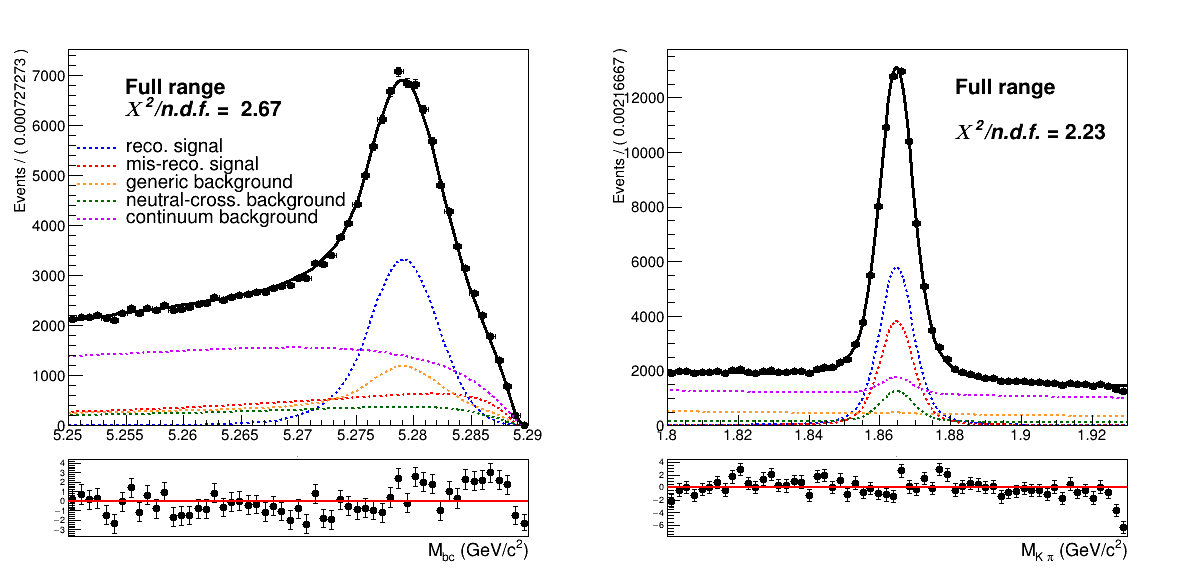
\includegraphics[width=0.80\textwidth]{05-chargedControlSample/figs/chargedControlD0_Total_2DFit_onData_paramCrossfeedRatio.png}}
  \caption{Two dimensional fit on Data with parametrized normalization of crossfeed background}
  \label{fig:chargedControlD0_Total_2DFit_onData_paramCrossfeedRatio}
  \end{figure}
 

  \vspace{0.5 cm}
  \begin{table}
 \begin{tabular}{ |p{3cm}||p{3cm}| p{3cm}|  }
 
  \hline
  ratio        &          MC      &    DATA   \\
  \hline
  \hline
 NmisSig/NrecSig  &  0.56 $\pm$ 0.01  & 0.66 $\pm$ 0.01\\
 NmisSig/Generic  &  0.90 $\pm$ 0.02 &  0.93 $\pm$ 0.02  \\
 Generic/NrecSig & 0.62 $\pm$ 0.01 & 0.71 $\pm$ 0.02\\
  \hline
 
 \end{tabular}
  \caption{Comparison of ratios of yields from the two dimensional fits on Monte Carlo simulated data and on Data (from the fit shown in \cref{fig:chargedControlD0_Total_2DFit_onData_paramCrossfeedRatio}).} 
  \end{table}




\newpage 
\subsection{Probability Density Functions (PDFs) for the $B_{tag}$}
Like for the signal model in the 2D fit the $M_{bc}$ distribution of the tagged charged $B$ mesons is fitted with a Crystal Ball as for the reconstructed  signal component, whereas the misreconstructed signal component is fitted with a Novosibirsk function (Fig. \ref{fig:stream0_chargedBtagFit_400bins_fixed_old_parameters_freeSigmaCB_and_misRecoPdf}).

\begin{figure}[H]
\begin{minipage}{.5\textwidth}
\centering
\subcaptionbox{\label{fig:stream0_chargedBtagFit_400bins_fixed_old_parameters_freeSigmaCB_and_misRecoPdf}}
{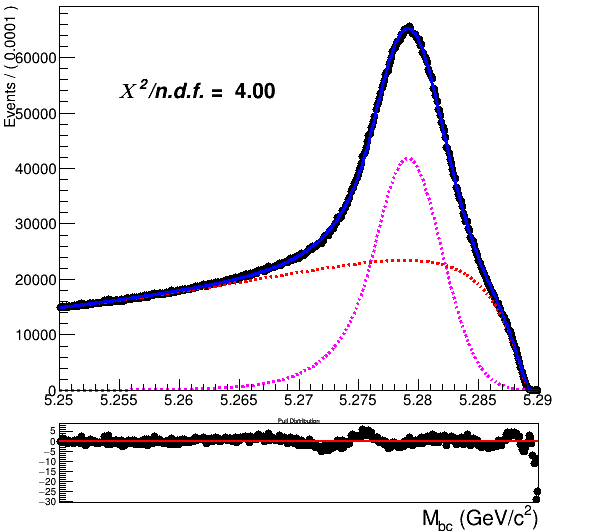
\includegraphics[width=0.80\textwidth]{05-chargedControlSample/figs/stream0_chargedBtagFit_400bins_fixed_old_parameters_freeSigmaCB_and_misRecoPdf.png}}
\end{minipage} 
 \begin{minipage}{.5\textwidth}
\subcaptionbox{\label{fig:NeutralCrossfeed_stream0_ControlD0_chargedBtag_MbcFit}}
{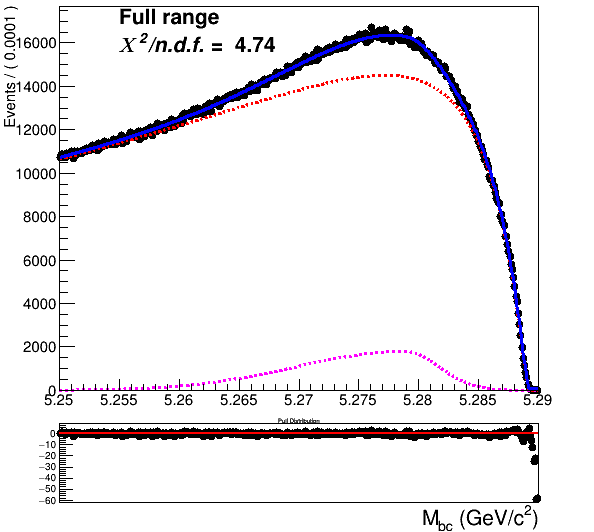
\includegraphics[width=0.80\textwidth]{05-chargedControlSample/figs/NeutralCrossfeed_stream0_ControlD0_chargedBtag_MbcFit.png}}
\end{minipage}
\caption{On the left: fitted distribution of tagged charged $B$ mesons, reconstructed signal events (magenta) are described by a Crystal Ball whereas the misreconstructed signal events (red) are described by a Novosibirsk function. On the right: Crossfeed distribution fitted with a sum of Novosibirsk (red) and asymmetric Gaussian PDF (magenta)}
\end{figure}


\noindent The crossfeed background is fitted instead with a sum of a Novosibirsk and an asymmetric Gaussian PDF (Fig. \ref{fig:NeutralCrossfeed_stream0_ControlD0_chargedBtag_MbcFit}).\\
\vspace{0.05 cm}

\noindent Regarding the continuum background component, same procedure used for the 2D fit was applied to the $M_{bc}$ distribution of the continuum background in this case (see Fig. \ref{fig:bin_corrected_stream1_off-resonance_on_stream3_on-resonance} for the result).

\begin{figure}[H]
\begin{minipage}{.5\textwidth}
  \centering
  {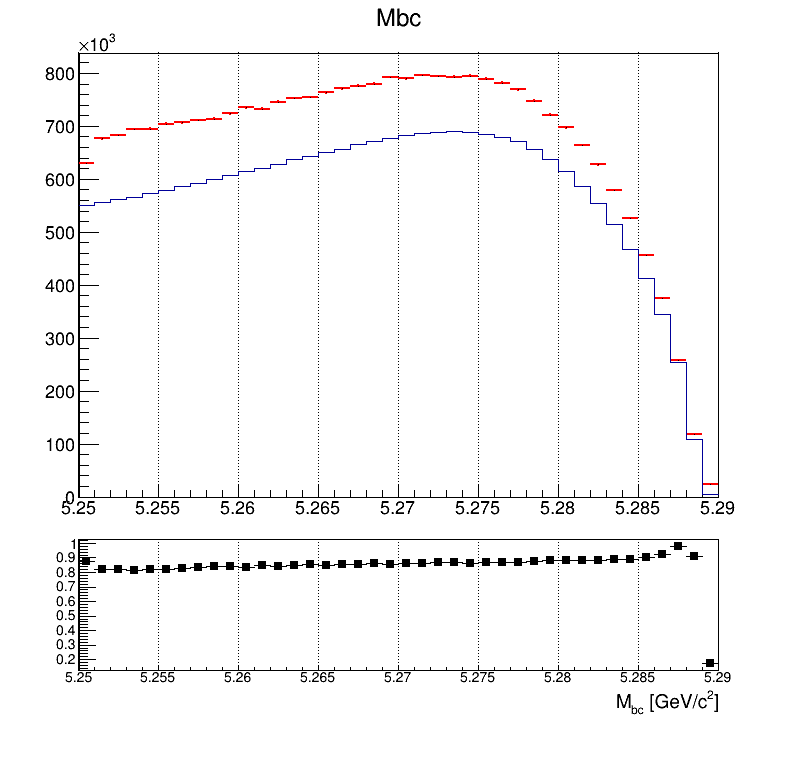
\includegraphics[width=0.80\textwidth]{05-chargedControlSample/figs/NEWstream0_chargedBtag_rescaled_off-on_resonance.png}}
%\caption{}
%\label{fig:NEWstream0_chargedBtag_rescaled_off-on_resonance}
\end{minipage}%
\begin{minipage}{.5\textwidth}
%\centering
{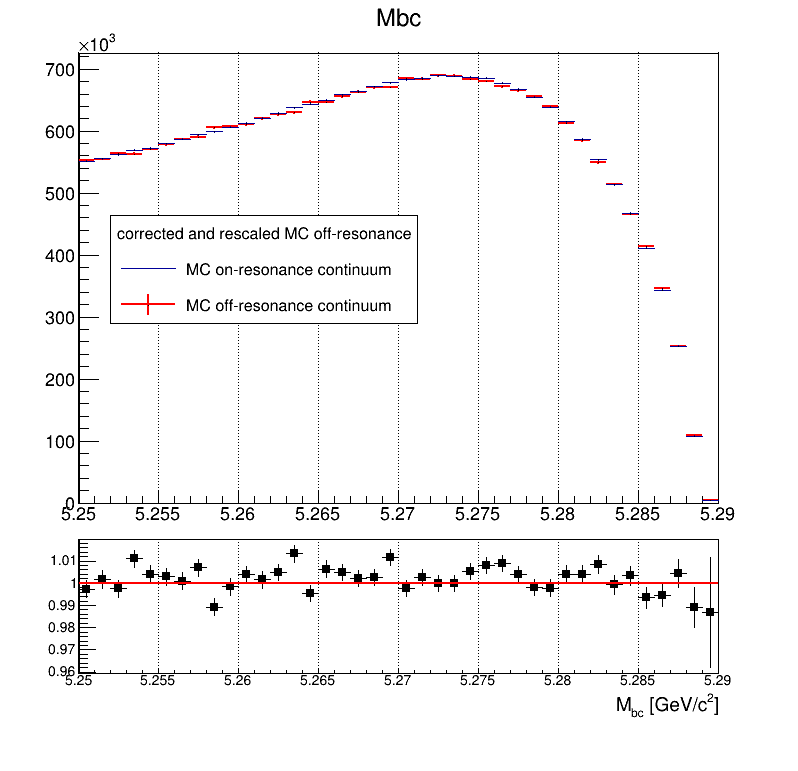
\includegraphics[width=0.80\textwidth]{05-chargedControlSample/figs/bin_corrected_stream1_off-resonance_on_stream3_on-resonance.png}}
%\caption{}
\label{fig:bin_corrected_stream1_off-resonance_on_stream3_on-resonance}
\end{minipage}
\caption{On the left: $M_{bc}$ distributions of the MC off-resonance sample and the MC continuum sample. On the right: $M_{bc}$ distributions of the corrected scaled MC off-resonance and on-resonance MC continuum.}
\end{figure}


\subsection{$B_{tag}$ Fit on Monte Carlo simulated data}

An independent Monte Carlo stream was used to test the total fit model on tagged $B$ mesons candidates. 
The usual condition is applied to the crossfeed background events: the ratio between its contribution and misreconstructed signal events is fixed from the other Monte Carlo stream.\\
In this fit the shaping parameters that are not kept fixed are the Crystal Ball width ($\sigma_{CB}$) and the width of the Novosibirsk function describing the misreconstructed signal events.
As in the case of $B_{tag}$ fit in Sec. \ref{BtagFit} the range for the fit is restricted to values betweeen 5.250 and 5.287 GeV/$c^2$.   





\begin{figure}[H]
\begin{minipage}{.5\textwidth}
  \centering
  {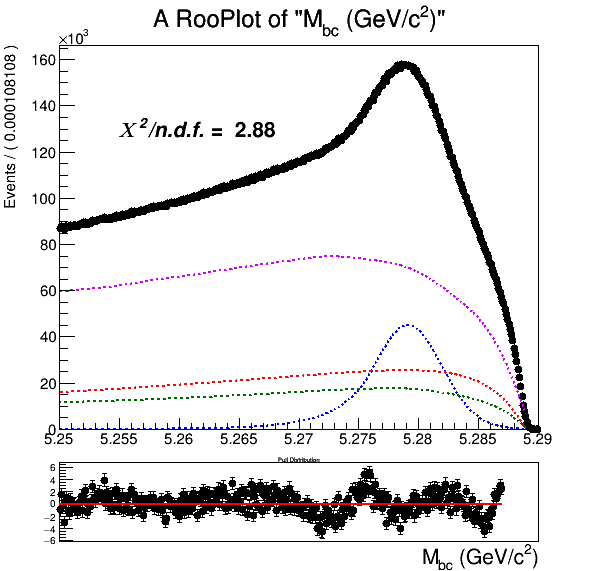
\includegraphics[width=0.95\textwidth]{05-chargedControlSample/figs/stream3_chargedBtag_Total_fit_sigmaCB_misRecSigma_free_370bins.png}}
%\caption{}
%\label{fig:NEWstream0_chargedBtag_rescaled_off-on_resonance}
\end{minipage}%
\begin{minipage}{.5\textwidth}
%\centering
{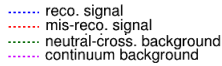
\includegraphics[width=0.55\textwidth]{05-chargedControlSample/figs/legend.png}}
%\caption{}
%\label{fig:bin_corrected_stream1_off-resonance_on_stream3_on-resonance}
\end{minipage}
\caption{Total fit of tagged $B$ mesons}
\end{figure}


Yields for the reconstructed and misreconstructed signal are obtained from the fit:

\vspace{0.5 cm}
\begin{tabular}{ |p{2cm}||p{3.8cm}|  }

 \hline
 NrecSig  & 3.25110$\cdot$10$^6 \pm$ 6759\\
 NmisSig &  7.41107$\cdot$10$^6 \pm$ 5341 \\
 \hline
\end{tabular}



\vspace{0.5 cm}
\noindent  One can then compare the  sum  NrecSig+NmisSig (the so called total signal) with the true value known from the Monte Carlo and the same for the total number of events in this particular stream: \\
 %The Total normalization from the fit is 38600851 $\pm$  6886 (to be compared with 38609945 from the Monte Carlo).


\begin{tabular}{ |P{3cm}||P{4cm}|P{2cm}|  }

\hline
      & fit & MC value\\
 \hline
 Total Signal  & 10.662$\cdot$10$^6$ $\pm$ 5249 & 10.671$\cdot 10^6$ \\
 Total events &  38.601$\cdot$10$^6$ $\pm$ 6886 & 38.610$\cdot 10^6$\\
 \hline
\end{tabular}
\vspace{0.75 cm}
\newline
\noindent The discrepancy in the total signal events from the fit and the MC here is about 1.7$\sigma$, but the relative error is an order of magnitude smaller than the one found in $B_{tag}$ fit in \ref{BtagFit} (below the \textperthousand level), therefore it's negligible.

\newpage

\subsection{$B_{tag}$ Fit on data}
The fit model tested on Monte Carlo simulated data is then applied with the same method on data \cref{fig:chargedControlD0Btag_Total_fit_onData}.

\begin{figure}[H]
\centering
{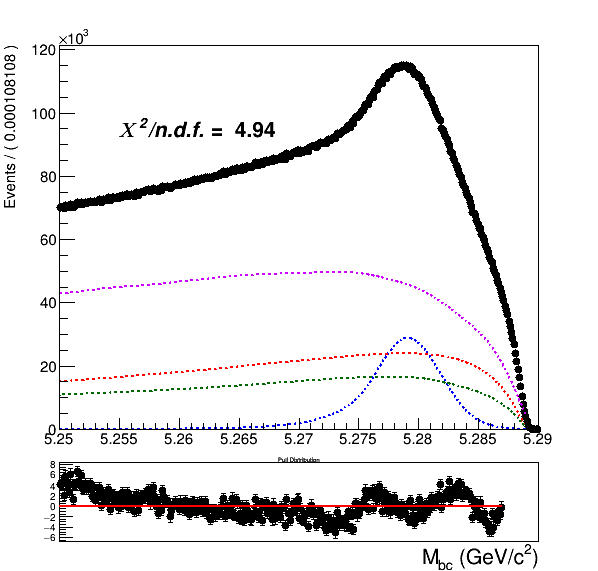
\includegraphics[width=0.40\textwidth]{05-chargedControlSample/figs/chargedBtag_Total_fit_onData_sigmaCB_free_370bins.png}}
\caption{Total fit of tagged $B^+$ mesons candidates on data}
\label{fig:chargedControlD0Btag_Total_fit_onData}
\end{figure}


Yields for the reconstructed and misreconstructed signal are obtained from the fit:

\vspace{0.5 cm}
\begin{tabular}{ |P{3cm}||P{4cm}|  }

 \hline
 NrecSig  & 2.011$\cdot$10 $^6 \pm$ 5858\\
 NmisSig &  6.975$\cdot$10 $^6 \pm$ 4667 \\
Total Signal &  8.982$\cdot$10 $^6 \pm$4587             \\
 \hline
\end{tabular}

  \vspace{0.5 cm}
  \begin{table}[H]
 %     \centering
\begin{tabular}{ |p{3cm}||p{3cm}|  p{3cm}| }

 \hline
 ratio        &          MC      &    DATA   \\
 \hline
NmisSig/NrecSig  &  2.28 $\pm$ 0.01  & 3.47 $\pm$ 0.01\\
 \hline  
 \end{tabular}
 \caption{Comparison of ratios of yields from the tagged $B$ mesons fits on Monte Carlo simulated data and on Data.}
\end{table}
 
\newpage

 \subsection{PID efficiency correction}\label{sec:ControlPIDeff}

The PID selection is applied only to Kaons: $\frac{\mathcal{L}_{K}}{\mathcal{L_{K}}+\mathcal{L_{\pi}}} > 0.6$ 
%The kaon identification efficiency  was studied in detail Belle Note 779 (\url{http://belle.kek.jp/secured/belle_note/gn779/bn779.ps.gz}). The decay $D^{*+} \rightarrow D^0 \pi^+$ followed by $D^0 \rightarrow K^- \pi^+$, was used to examine the Kaon identification efficiency difference between data and MC in \textit{Belle}.
%The efficiency ratio dependence on Kaon charge, momentum and polar angle is considered. 
%As already The Kaon ID efficiency is defined as\\

%\vspace{0.2cm}
%\hspace{3 cm}    $\epsilon_{KID} = \frac{\text{number of}\hspace{0.05 cm}K \text{tracks identified as} \hspace{0.05 cm} K}{\text{number of }K \hspace{0.05 cm} \text{tracks} }$\\

%\vspace{0.2cm}
% and the comparison between MC efficiency and data efficiency by a double ratio defined as \\

%\vspace{0.2cm} \hspace{1 cm}  $ R = \epsilon^{data}/\epsilon^{MC}$ \\

\vspace{0.5cm}
Using the values provided in the global tag \texttt{BellePID} (as done in the $\BtoLambda$ study), the average Kaon ID correction for this analysis is estimated to be $R = 0.976 \pm 0.008$.



\subsection{$D^0$ and FEI efficiency}\label{sec:ControlRecoEff}

The efficiency in reconstructing the $D^0$ after correctly tagging the charged $B$ meson, can be estimated from the 2D fit on Monte Carlo simulated data, using the reconstructed signal yield and from a sample of $B_{tag}$ candidates reconstructed in signal events in the Monte Carlo: where from $B^+ B^-$ at least a $D^0$ decaying into $\pi K$ is produced.

For the latter a fit is performed to extract the yield of correctly tagged $B$ mesons (Fig. \ref{fig:stream0_chargedBtagSignal_fit})
\begin{figure}[H]
\centering
{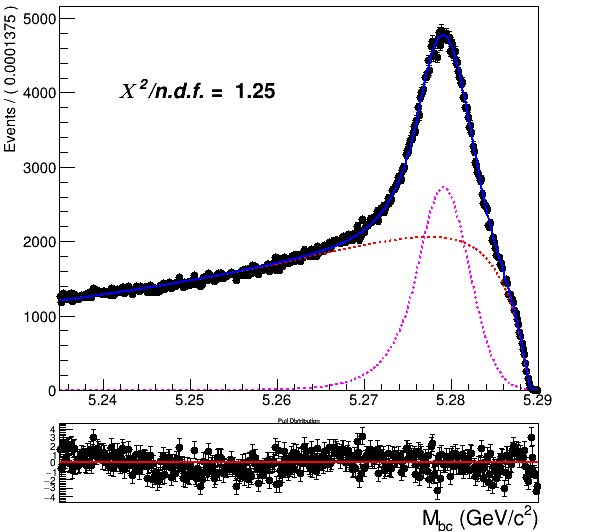
\includegraphics[width=0.40\textwidth]{05-chargedControlSample/figs/stream0_chargedBtagSignal_fit.png}}
\caption{Fit of tagged $B$ mesons in the "signal events" sample}
\label{fig:stream0_chargedBtagSignal_fit}
\end{figure}

Yields for the reconstructed and misreconstructed signal :

\vspace{0.5 cm}
\begin{tabular}{ |P{2cm}||P{4cm}|  }

 \hline
 NrecSig  & 1.46779$\cdot$10 $^5 \pm$ 767\\
 NmisSig &  6.16717$\cdot$10 $^5 \pm$ 1028 \\
 \hline
\end{tabular}
\vspace{0.5 cm}

\noindent From this and the results listed in Sec. \ref{2Dfit_chargedControlD0_onMC} 
the efficiency to reconstruct $D^0$ is obtained : \\

$\epsilon_{D^0} = \frac{NrecSig(2D) }{NrecSig((B_{tag}^{sig}} = 39.1 \pm 0.4 \%\footnote{the error reflects the limited Monte Carlo statistics}$  \hspace{0.4cm} (KID efficiency corrected value for data: 38.2 $\%$)\\
\vspace{0.2 cm}

\noindent The results from the fit shown in  (Fig. \ref{fig:stream0_chargedBtagSignal_fit}) can be used also to calculate the FEI tag-side efficiency for signal events, i.e. the efficiency to tag the $B$ meson accompanying a $B_{sig}$ decaying into a $D^0 $ on the signal side.
Whereas results from the fit  of charged $B_{tag}$ shown in Fig. \ref{fig:stream0_chargedBtagFit_400bins_fixed_old_parameters_freeSigmaCB_and_misRecoPdf} can be used to calculate the hadronic tag-side efficiency in the generic $B^+B^-$ events case.

\noindent The ratio of the two efficiencies is found to be:   $\frac{\epsilon^{+}_{FEI,  sig}}{\epsilon^{+}_{FEI}} = 1.50 \pm 0.01 $ \\
\vspace{0.2 cm}

\subsection{Studies of Systematic Effects}\label{sec:chargedControlSys}

The systematic uncertainties are studied the same way as in the case of the $B^+ \rightarrow \bar{\Lambda}_c^- X$ branching fraction. 
The values are reported in the next section. The dominant systematic uncertainty is the one originated by the continuum background modeling and its incidence in terms of relative error on the branching fraction value is same as for the $B^+ \rightarrow \bar{\Lambda}_c^- X$ study.
For this control sample study the uncertainty that would be caused by the uncertainty of the crossfeed peaking events is not estimated, since 
the uncertainty on   $\mathcal{B}(B^0 \rightarrow \bar{D^0} + X)$ is only of few percent and the possible effect can be considered negligible compared to the other systeamtic uncertainties. 


\subsection{Measured $B^+ \rightarrow \bar{D}^0 X$ inclusive Branching Fraction}\label{sec:chargedControlBRvalues}
The inclusive branching fraction of $B^+  \rightarrow \bar{D}^0 X$ can be determined by: 

\begin{equation}
    Br(B^+ \rightarrow \bar{D}^0) = \frac{r}{Br(D^0 \rightarrow K^+ \pi^-) \epsilon_{D^0}}  \cdot  \frac{\epsilon^{+}_{FEI}}{ \epsilon^{+}_{FEI,  sig} }
\end{equation}

Where 
\begin{itemize}

\item $r = \frac{N_{tag, D^0}}{N_{tag}}$ is the ratio of reconstructed signal yield in the two dimensional fit and in the $M_{bc}$ fit of the tagged $B$ mesons.
\item $\epsilon_{D^0} $ is the $D^0$ reconstruction efficiency calculated as fraction of reconstructed signal events with correct tag of which then also a correctly reconstructed $D^0$ is reconstructed in the signal side.
\item $\frac{\epsilon^{+}_{FEI}}{ \epsilon^{+}_{FEI,  sig }}$ is the ratio of the FEI efficiencies: the hadronic tag-side efficiency for generic $B^+B^-$ events ($\epsilon^{+}_{FEI}$) and signal-side depedent one ($\epsilon^{+}_{FEI,  sig}$)  where one of the two $B$ mesons decays inclusively into the signal channel ($D^0 \rightarrow K^+ \pi^- $) 
\item  $Br(D^0 \rightarrow K^+ \pi^-) = 3.8\% $ in Belle DECAY.DEC table,
$Br(D^0 \rightarrow K^+ \pi^-) = 3.95\% $ in PDG.
\end{itemize}

\vspace{0.2 cm}


In Monte Carlo:  \hspace{0.05cm} $Br(B^+ \rightarrow \bar{D}^0) = 79.4 \pm 0.6^{(stat.)} \%$ \hspace{1cm}  (true MC value: $79.1\%$) \\ % \pm 0.5^{(stat.)} \%$) \\
\vspace{0.25 cm} \newline
\hspace{0.1cm}  $ $ As for the Data, the value obtained using a fixed ratio of crossfeed events with respect to misreconstructed signal events is:
  \hspace{0.05cm} $Br(B^+ \rightarrow \bar{D}^0) = 78.3 \pm 0.8^{(stat.)} \%$ \\
  \vspace{0.25 cm} \newline
  While, introducing the parametrization of the crossfeed normalization in the two dimensional fit gives a larger value:  \hspace{0.05cm} $Br(B^+ \rightarrow \bar{D}^0) = 80.3 \pm 0.8^{(stat.)} \%$ \\
  \vspace{0.25 cm}
  \noindent Nevertheless, the latter is in agreement with the value reported by the PDG:  ($79 \pm 4)\%$\\%
  One can conclude that the obtained results have proven the validity of  the method chosen for the measurements.
  %\hspace{1cm}  
  

%\vspace{0.2 cm}
 %KID efficiency corrected:

\vspace{0.2 cm}
\noindent The systematic uncertainties are dominating as one can see from the Table below, listing the contribution of the various sources of systematics in terms of Branching Fraction in percentage.\\
%\vspace{0.1 cm}


%\textbf{systematics:}\\
\vspace{0.1 cm}
\begin{table}[H]
\label{tab:chargedControlSyst}
\centering
\begin{tabular}{c|c}
 continuum   modelling & 1.8 $\%$\\
Crossfeed PFDs    & 0.4 $\%$\\
Crossfeed fraction      &  0.8 $\%$ \\
2DFit crossfeed normalization & 0.4 $\%$ \\
 FEI efficiency    & 0.5 $\%$ \\
   $\epsilon_{D^0} $   & 0.8 $\%$ \\
 PID    & 0.6 $\%$ \\
 Tracking efficiency  & 0.8 $\%$\\
 \hline
 Total & 2.5 $\%$
\end{tabular}

\caption{Sources of systematic uncertainties and their contributions.}

\end{table}
